\chapter{Noise Filtering}\label{NoiseFiltering}
\section{Research}
\subsection{Voice frequency analysis}
Voice frequency ranges vary heavily depending on whether it sources from a male of a female. Fundamental voice frequency varies from 100Hz to 900 Hz for men and 350Hz to 3KHz for women. Including peaks to conserve natural sounding voice, a wider frequency range has to be considered. It rises to 8 KHz for males and 17KHz for females. \cite{Seaindia}. Yet different researches often come up with different results. For example, in phone communications it is accepted to transmit frequency range between 400Hz and 3400Hz. This is the reason some peoples' voices transit poorly over the phone yet for most cases it work fine. This example allows to conclude that smaller frequency ranges could be acceptable. To conserve all of the properties of the human voice, filter boundaries should be around 100Hz to 17KHz but this range would filter out any noise as it takes up almost an entire frequency range of human hearing (approximately 20Hz to 20KHz).  
\subsection{Filtering characteristics}
\subsection{Results}
Making a field researh to find the frequency range that would fit the needs of this project was out scope, therefore to test the filters it was decided to take trial-error approach. A few samples were made outside during a windy day. This was considered a good idea as it has recreated one of the most common conversation scenarios.
At first it was attempted to conserve the entire frequency range that humans can produce. This has resulted in a filter that seemed to filter out a big part of the noise but if it was listened to, all of the previously recorded noise was still there.It was hard to tell the difference between filtered and not filtered sound samples.
\begin{figure}
  \centering
    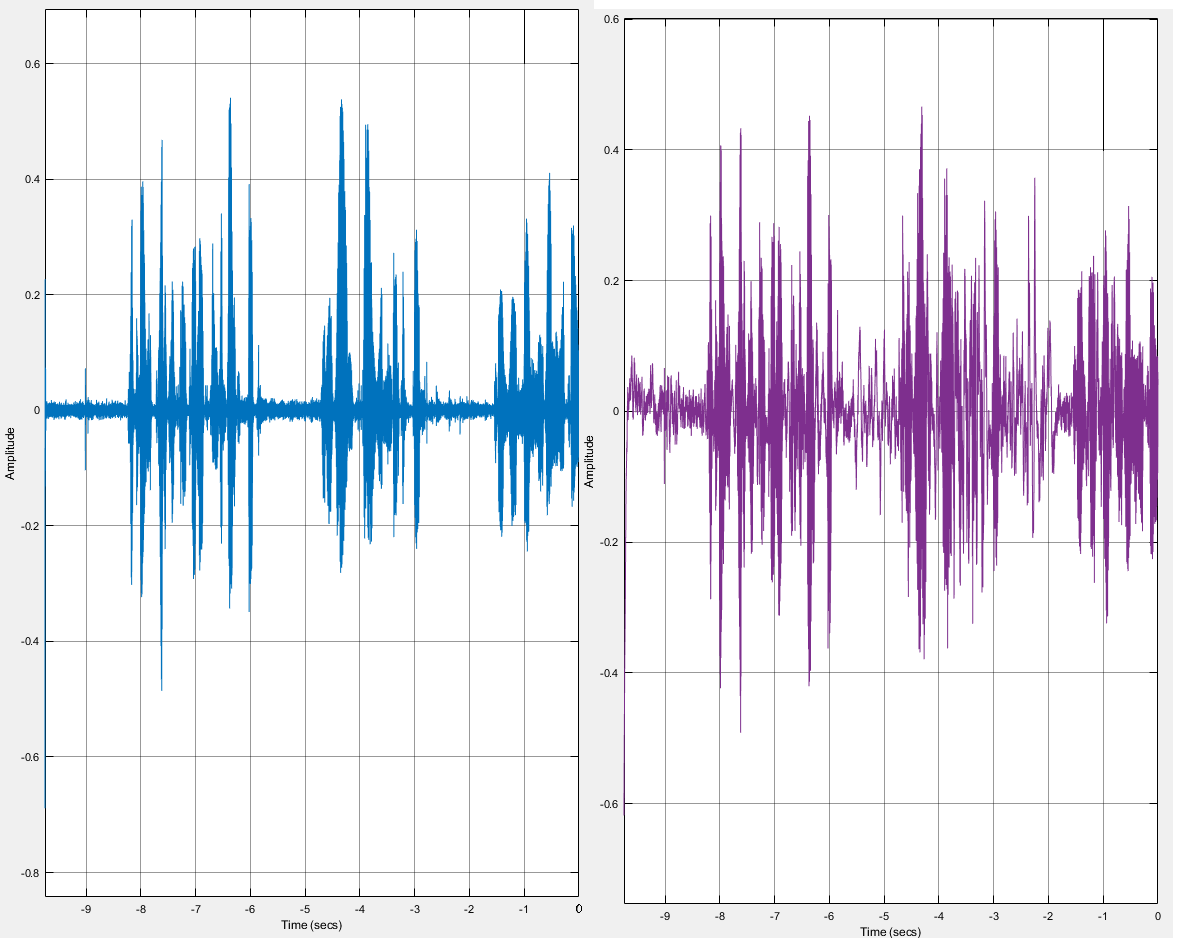
\includegraphics[width=0.7\paperwidth]{Illustrations/100HZto17KHzfilter}
    \caption{Filtered result on the left and recorded sample on the right}
\end{figure}

  